\begin{figure}[t]
  \centering
  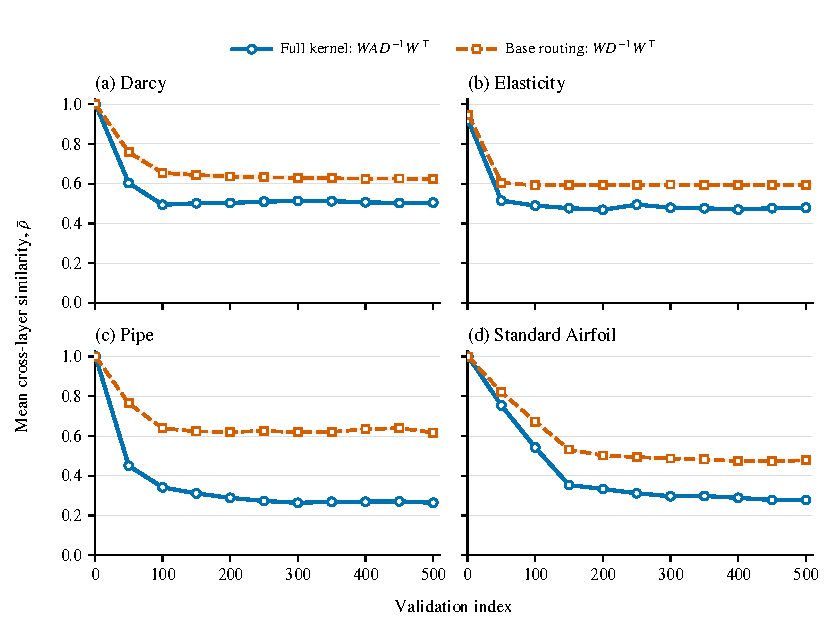
\includegraphics[width=\linewidth]{four_dataset_similarity_trajectories.pdf}
  \caption{\textbf{Evolution of cross-layer propagation-kernel similarity.}
  Mean off-diagonal Frobenius cosine similarity $\rho_{ij}$ between the
  propagation kernels of different Transolver blocks on four PDE benchmarks.
  The base kernel $P^{\mathrm{base}}=WD^{-1}W^\top$ measures the
  slice/deslice routing, whereas the full kernel
  $P^{\mathrm{full}}=WAD^{-1}W^\top$ additionally includes attention
  between slice tokens. Higher similarity indicates less differentiated
  spatial propagation across blocks. Curves report the mean over four
  monitored samples and shaded regions denote one standard deviation.
  Cross-layer heads are compared by optimal bipartite matching, making the
  metric invariant to head permutations. Each validation index corresponds
  to one training epoch in these experiments.}
  \label{fig:cross-layer-kernel-similarity}
\end{figure}
